\documentclass[12pt, letterpaper]{article}
\usepackage[english]{babel}

% margins
\usepackage[a4paper, margin=2.5cm]{geometry}

% include pdf
\usepackage[final]{pdfpages}

% fix line breaks urls
\PassOptionsToPackage{hyphens}{url}
\usepackage[hidelinks]{hyperref}

\usepackage{graphics}

% Special/larger tables
\usepackage{longtable}
\usepackage{tabularx}

% quotes
\usepackage{csquotes}

% Acronyms
\usepackage[nopostdot,style=super,nonumberlist,toc,nogroupskip,acronym]{glossaries}

% For typesetting
\usepackage{lipsum}  

% Double spacing
\usepackage{setspace}

% appendix
\usepackage[page, title]{appendix}

% tables
\usepackage{booktabs}
\usepackage{array} % centering + width fix

\usepackage{caption} 
\captionsetup{labelfont=bf,labelsep=period,font=footnotesize,}
\usepackage{cleveref}

% Fix section titles size/format
\usepackage{titlesec}
\titleformat{\section}
  {\normalfont\fontsize{16}{21}\bfseries}
  {\thesection}
  {1em}
  {}

\titleformat{\subsection}
  {\normalfont\fontsize{14}{18}\bfseries}
  {\thesubsection}
  {1em}
  {}

  \titleformat{\subsubsection}
  {\normalfont\fontsize{12}{14}\itshape}
  {\thesubsubsection}
  {1em}
  {}

\titlespacing{\section}{0pt}{\parskip}{-\parskip}
\titlespacing{\subsection}{0pt}{0.75\parskip}{-\parskip}
\titlespacing{\subsubsection}{0pt}{0.5\parskip}{-\parskip}

% Remove section numbers
\setcounter{secnumdepth}{0}

% Set paragraph spacing
\setlength{\parindent}{0pt}
\setlength{\parskip}{1em}
\def\ni{\noindent}

%% These two lines are needed to get the correct paper size
%% in TeX Live 2016
\let\pdfpageheight\paperheight
\let\pdfpagewidth\paperwidth

\makenoidxglossaries

\newacronym{auc}{AUC}{area under the receiver operating characteristic curve}
\newacronym{mam}{M\&M}{morbidity and mortality}
\newacronym{ml}{ML}{machine learning}
\newacronym{ofi}{OFI}{opportunity for improvement}
\newacronym{qi}{QI}{quality improvement}
\newacronym{gan}{GAN}{generative adversarial network}
\newacronym{iss}{ISS}{injury severity score}
\newacronym{swetrau}{SweTrau}{Swedish Trauma Registry}
\newacronym{ci}{CI}{confidence interval}
\newacronym{ctgan}{CTGAN}{conditional tabular generative adversarial network}
\newacronym{tvae}{TVAE}{triplet based variational autoencoder}
\newacronym{vae}{VAE}{variational variable autoencoder}

\newglossaryentry{trauma}
{
    name=Trauma,
    text=trauma,
    description={Damage inflicted on the body as the direct or indirect result of an external force, with or without disruption of structural continuity.}
}

\newglossaryentry{gofi}
{
    name={OFI},
    text={OFI},
    description={Short for opportunity for improvement, is a consensus reached at a morbidity and mortality conference regarding whether there exists opportunity for improvement in the handling of a singular patient trauma care.}
}



% Acronym style
\newglossarystyle{csuper}{%
    \setglossarystyle{super}%
    \renewcommand{\glossentry}[2]{%
        \glsentryitem{##1}\glstarget{##1}{\glossentryname{##1}} &
        \Glossentrydesc{##1}\glspostdescription\space ##2\tabularnewline
    }
    \setlength{\glsdescwidth}{0.75\linewidth}
}

% Glossary style
\newglossarystyle{gsuper}{%
    \setglossarystyle{super}%
    \renewcommand{\glossentry}[2]{%
        \glsentryitem{##1}\glstarget{##1}{\glossentryname{##1}} &
        \Glossentrydesc{##1}\glspostdescription\space ##2\\[1em]
    }
    \setlength{\glsdescwidth}{0.65\linewidth}
}

% References
\usepackage[style=numeric,
    backend=biber,
    sorting=none,
    url=false,
    isbn=false,
    terseinits=true,
    giveninits=true,
    minnames=6,
    maxnames=6]{biblatex}

% Remove unwanted punctuations
\renewcommand*{\revsdnamepunct}{}
\renewcommand*{\finentrypunct}{}
\renewcommand*{\bibpagespunct}{}

% Dot instead av brackets in references
\DeclareFieldFormat{labelnumberwidth}{\mkbibbold{#1\adddot}}

% Lastname followed by initials format
\DeclareNameAlias{sortname}{family-given}
\DeclareNameAlias{default}{family-given}
\renewcommand*{\revsdnamepunct}{}

\DeclareSourcemap{%
    \maps[datatype=bibtex]{
        % Journal abbreviations
        \map[overwrite]{
            \step[fieldsource=shortjournal]
            \step[fieldset=journaltitle,origfieldval]
        }
    }
}

% remove in
\renewbibmacro{in:}{}
% remove pp
\DeclareFieldFormat*{pages}{#1}
% reformat doi
\DeclareFieldFormat*{doi}{\url{https://doi.org/#1}}
%remove quotation marks around title
\DeclareFieldFormat*{title}{#1}


\DeclareFieldFormat{journaltitle}{\mkbibemph{#1}\isdot}

% Provide three letter month names
\newcommand*{\shortmonth}[1]{
    \ifthenelse{\NOT\equal{#1}{}}{
        \ifcase#1\relax
        \or Jan
        \or Feb
        \or Mar
        \or Apr
        \or May
        \or Jun
        \or Jul
        \or Aug
        \or Sep
        \or Oct
        \or Nov
        \or Dec
        \fi
    }
}

\DeclareFieldFormat*{number}{\mkbibparens{#1}}

\DeclareFieldFormat*{date}{\thefield{year}}

% Code adapted from biblatex-nejm package

\renewbibmacro*{volume+number+eid}{
    \printfield{volume}%
    \setunit{}%
    \printfield{number}%
    \addcolon%
    \printfield{eid}%
}

\renewbibmacro*{issue+date}{
    \usebibmacro{date}
}

\renewbibmacro*{journal+issuetitle}{
    \usebibmacro{journal}%
    \iffieldundef{series}%
    \adddot%
    {}
    {\newunit%
        \printfield{series}}%
    \setunit{\addspace}%
    \usebibmacro{issue+date}%
    \setunit{\addsemicolon}%
    \usebibmacro{volume+number+eid}%
    \usebibmacro{issue}%
    \newunit}

% compress page numbers. E.g. XYZ-XAB -> XYZ-AB
\DeclareFieldFormat{postnote}{\mkcomprange[{\mkpageprefix[pagination]}]{#1}}
\DeclareFieldFormat{pages}{\mkcomprange{#1}}

% Compress ranges where lower limit > 100
\setcounter{mincomprange}{100}

% Don't compress beyond the fourth digit
\setcounter{maxcomprange}{1000}

% Display compressed upper limit with at least two digits,
% unless leading digit is zero
\setcounter{mincompwidth}{10} %imports biblatex 
\addbibresource{main.bib}


\begin{document}
\begin{titlepage}
    
\includepdf[pages=-,pagecommand={},fitpaper=true,]{title_page.pdf}
\end{titlepage}

\pagenumbering{Roman}

\textbf{Titel}

\lipsum[1]

\vfill

\textbf{Title}

\lipsum[1]

\vfill

\textit{Keywords}: Machine learning; Trauma; Medical audit; Trauma care quality improvement; Data synthesis; Prediction

\newpage

\glsaddall
\printnoidxglossary[type=acronym,style=csuper]
\printnoidxglossary[style=gsuper]

\newpage
\pagenumbering{arabic}

\setstretch{1.5}

\section{Introduction}
\Gls{trauma} is a major contributor to death and illness for individuals between the ages of 10 and 49 worldwide, and the leading cause of death amongst young people in Sweden \cite{roth_global_2018, vos_global_2020, sos_death_2021}. The \gls{trauma} population has a low average age and two-thirds of the group have no history of co-morbidity \cite{brattstrom_socio-economic_2015}. Thus it is essential to ensure a constant high-quality \gls{trauma} care to lower mortality and morbidity for this population with long a age expectancy.

A method of improving trauma patient care is to implement \acrfull{qi} programmes, as suggested by the World Health Organization (WHO) \cite{world_health_organization_guidelines_2009}. \Acrfull{mam} conferences are a cornerstone in such programmes and aim to identify \acrfull{ofi} in patient care \cite{santana_development_2014}. \acrshort{mam} conferences are conducted by representatives from all disciplines and professions involved in trauma care. During these conferences the treatment provided for an individual patient is discussed and compared against the optimal treatment that should have been provided. Regularly performing such reviews are associated with reducing complication frequencies, hospitalisation time, and preventable deaths; thus providing high-quality trauma care \cite{stelfox_evidence_2011, mcdermott_trauma_1994}. Due to the nature of \acrshort{mam} conferences however, they are extremely resource intensive \cite{}.

An \acrshort{ofi} is a concrete deficiencies in patient care and are often occur in initial care, such as, airway management, fluid resuscitation, haemorrhage control, and chest injury management \cite{world_health_organization_guidelines_2009,roy_learning_2017,oreilly_opportunities_2013,sanddal_analysis_2011}.

A more advanced \acrshort{qi} technique suggested by WHO is the application of audit filters that use electronic health record systems to monitor predefined variables to flag patient cases with \acrfull{ofi} \cite{world_health_organization_guidelines_2009}. Filtering cases using an audit filter before reviewing by an \acrshort{mam} conference provides a possibility to reduce false positive cases and thus reducing the costs of the \acrshort{qi} programme as a whole.

However, the performance of such systems varies and have been associated with high frequencies of false positives. Depending on context the frequency of false positives can range from 24\% to 80\% \cite{attergrim_predicting_2023,sanddal_analysis_2011,roy_learning_2017,ghorbani_analysis_2018}.

A new method suggested by Attegrim and Szolnoky et al. suggests to replace audit filter systems with supervised \acrfull{ml} models \cite{attergrim_predicting_2023}. These newer models achieve a significantly better performance than the currently used audit filter system at Karolinska University Hospital in Stockholm, Sweden. At the same sensitivity, the false positive rate is reduced from 68\% to 53\% using the same data.

Despite this performance boost, the models' still suffer from that 50\% of patient cases are incorrectly flagged as \acrshort{ofi} positive. \acrshort{ml} methods in general require large amounts of data to be able to perform \cite{piccialli_survey_2021}. Many methods exist to increase the performance of \acrshort{ml} models, and perhaps the most fundamental and well known is simply increasing the sheer amount of data. So far, the only possible method in doing so was by manually collecting more data and annotating it. This is a slow process, and in some cases not possible due to the fundamental lack of data.

\begin{figure}[t]
    \centering
    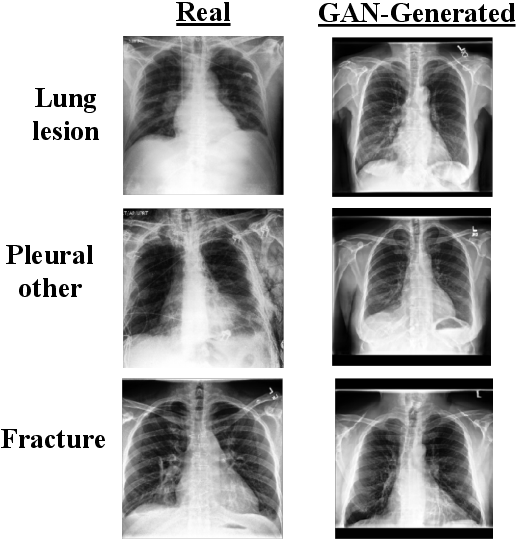
\includegraphics[width=0.6\textwidth]{figures/gan-xray.png}
    \caption{Example of using a \acrfull{gan} to generate chest radiograph images. Image taken from \cite{sundaram_gan-based_2021}.}
    \label{fig:gan-xray}
\end{figure}

Recently however, using \acrfullpl{gan} to generate synthetic data has become a hot topic in image analysis \cite{pavan_kumar_generative_2021}. See \Cref{fig:gan-xray} for an example usage of \acrshortpl{gan} in image analysis. A \acrshort{gan} is a type of artificial neural network. It consists of two main parts: a generator and a discriminator. The generator is trained to produce new data samples that are similar to the input data, while the discriminator is trained to distinguish between the generated samples and the real data. The generator and discriminator are trained together, in an adversarial manner: the generator tries to produce samples that the discriminator cannot correctly identify as fake, while the discriminator tries to correctly identify the fake samples produced by the generator. Through this process, the generator learns to produce samples that are similar to the input data, and the discriminator learns to recognize the differences between the real and generated data. Thus the two generator constantly evolves to be able to produce data more closely to the source that the discriminator cannot differentiate as synthetic data.


%\acrshortpl{gan} internally use two neural networks, one network to generate data (the generator) and another that tells how realistic the data is compared to the ground truth data (the discriminator). During the training of \acrshortpl{gan}, the two internal models constantly compete; the generator model generating data that the discriminator can't tell apart from the ground truth data \cite{}. \acrshortpl{gan} can be seen as a sort of evolutionary arms race between the two internal models, similar to the evolutionary process known as mimicry. In short,by training a \acrshort{gan} on true manually annotated data one can there after produce more data.

Another form of artificial neural network generative models are the \acrfull{vae} \cite{kingma_auto-encoding_2013}. It is a simpler and more compact model that works by learning the probabilistic representation of a dataset, called the latent space. The latent space can simply be described as a compressed representation of the input data that captures the most important features and variations in the data. The \acrshort{vae} consists of two main parts: an encoder and a decoder. The encoder takes in the input data and maps it to a probability distribution in the latent space, while the decoder takes a sample from this distribution and maps it back to the original data space. By training the \acrshort{vae}, we can learn a compact representation of the input data that captures the most important features and variations in the dataset.


The quality of the generated data often varies and depends on several factors, such as, the quality and amount of ground truth data \cite{karras_training_2020}. The major benefit of having a method for generating quality synthetic data is the possibility of expanding small datasets and training \acrshort{ml} models where it was not previously possible or did not achieve adequate results due to data amount.

In addition to generating more trainable data, some \acrshortpl{gan} are able to anonymise data \cite{liu_ppgan_2019}. Thus providing an interface for being able to generate synthetic datasets of sensitive personal information that are completely anonymous. These synthetic datasets can, in theory, be distributed and increase the availability of medical datasets for researchers.

\subsection{Aim}
Hitherto, using \acrshortpl{gan} is rare and relatively unexplored for structured tabular data. Few articles exist investigating the feasibility of generating synthetic tabular data in a medical context.

Therefore, the aim of this article is to evaluate the effectiveness of using \acrshortpl{gan} for generating synthetic tabular data in a trauma setting, and to investigate the potential of this approach for improving \acrshort{ofi} prediction models.

\section{Materials and Methods}
We conducted a retrospective study using registry data from Karolinska University Hospital, comparing the performance of supervised machine learning models that were trained with synthetic data and those that were not, by analysing all trauma patients in the trauma registry and quality database from 2014 to 2021.

The code used in this study is available online at \url{https://codeberg.org/kelszo/ofi-synthesiser} under the \textit{GNU Affero General Public License v3.0} license.

\subsection{Study Population and Setting}
Karolinska University Hospital in Solna, Sweden manages approximately 1500 acute trauma patients per year making it equivalent to a level 1 trauma center. The hospital reports all patients admitted with an \acrfull{iss} score more than 9, as well as, all patients admitted with trauma team activation regardless of \acrshort{iss} score to the \acrfull{swetrau} \cite{swetrau}. \acrshort{swetrau} inlcudes data on patient parameters, such as, blood pressure, heart rate, and respiratory rate, as well, injuries, interventions, and various checkpoint times. The registry is compliant with the Utstein template for uniform reporting of data following major trauma \cite{ringdal_utstein_2008}.

Parallel with this registry Karolinska University Hospital maintains an internal \acrshort{qi} registry known here as the quality database. The quality database includes data relating to the \acrshort{qi} program and \acrshort{mam} conferences, such as, audit filter results, identified \acrshortpl{ofi} and their recommended corrective actions. For all currently used audit filters at Karolinska University Hospital see \Cref{tab:auditfilters} in the appendix.

The Karolinska University Hospital conducts multidisciplinary conferences to review the outcomes of trauma patients, involving all healthcare professionals involved in their initial care, this includes surgery, anaesthesia, orthopaedics, intensive care, radiology, and nursing. \acrshort{ofi} are identified through a consensus decision, and appropriate corrective actions are suggested. Mortality cases immediately escalated to the mortality conference while morbidity cases includes escalating levels of reviews. Mortality conferences conclude whether a patient mortality was preventable or possibly preventable. The review process for morbidity cases was improved and formalized during the study period, with audit filters applied to the trauma quality database and individual reviews by specialised nurses were added in 2017. Between years 2014 and 2017, a specialised trauma nurse selectively reviewed trauma patients to identify possible \acrshortpl{ofi} to escalate to a \acrshort{mam} conference. Following 2017, a specialised nurse registered data to the trauma registry while at the same time looking for possible audit filter violations (including a possible manual violation flag) and applying them to the trauma quality database. If a violation was detected, the patient was reviewed again by two specialised nurses. If the second review could not exclude a possible \acrshort{ofi} the patient case was finally escalated to a morbidity conference for a final verdict.

All patients screened for \acrshort{ofi} between 2014 and 2021 were included. Patients under the age of 15 were excluded due to differing clinical pathway.

\subsection{Predictor Variables}
All variables included in the trauma registry and the revised Utstein template for major trauma were used as predictors for both \acrshort{ofi} classification and data synthesising \acrshort{ml} models. The predictors included both categorical and continuos values, including but not limited to, blood pressure, interventions, injury mechanisms and intentions, care length and level, and time points. The trauma registry includes data for the whole patient care, including pre-hospital setting and treatment, in-hospital care, and outcome in the form of Glasgow Outcome Scale and mortality. For a complete list of predictors, and their respective definitions, see the revised Utstein template for major trauma \cite{ringdal_utstein_2008} or \Cref{tab:predictors} in the appendix.

\subsection{Outcome variable}
The outcome was defined as the verdict from the \acrshort{mam} conference with the binary levels of "Yes - At least one \acrshort{ofi} identified" or "No - No \acrshort{ofi} identified". Preventable or possible preventable deaths were considered as an \acrshort{ofi}.

\subsection{Model Development and Data preprocessing}
All model development and data preprocessing was performed in Python. The model development can be separated in the development of the classification and synthesising models. For more specifics regarding implementation specifics, versions, and packages see the project source code.

\subsubsection*{Data preprocessing}
A pre-processor was developed to be able to pre-process both the training and test data without any leakage. This was done by rescaling continuous features using Yeo-Johnson's power transformation \cite{yeo_new_2000} and encoding nominal features using one-hot encoding. Ordinal features were left unchanged. Continuous features were imputed by using the mean of the feature, ordinal by using the most frequent value, and nominal by adding an "unknown" category. An exception was made for both the pre-hospital and emergency department blood pressure and respiratory rate, they were imputed by using the mean value of the revised trauma score category \cite{ringdal_utstein_2008}, if it existed. The pre-processor was trained and applied on the training data to be there after only applied to the test data, thus no data leakage occurred between the test and training set.

\subsubsection*{Classification models}
As suggested by Attegrim and Szolnoky et al. the following models were traditional methods were implemented with scikit-learn \cite{pedregosa_scikit_2011}: logistic regression, random forest, decision tree, support vector machine, k-nearest neighbour. The following boosting methods were implemented using the provided Python implementation: XGBoost \cite{chen_xgboost_2016}, LightGBM \cite{ke_lightgbm_2017}, and CatBoost \cite{prokhorenkova_catboost_2018}. Hyperparameter tuning was run all models, using the first resamples training data through a 5-fold cross validation. The suggested parameters, found either by the source documentation or implementation documentation, were optimised using Tree-structured Parzen Estimator \cite{bergstra_algorithms_2011} for a total of 1 hour per model.

\subsubsection*{Synthesising models}
The \acrfull{ctgan} \cite{xu_modeling_2019} and \acrfull{tvae} \cite{ishfaq_tvae_2018} models were implemented with the help of the Synthetic Data Vault framework \cite{patki_sdv_2016} available in Python. The batch size was increased to 1000 samples to include more minority cases in a single batch. Otherwise the standard parameters provided were used.

\subsection{Statistical Analysis}
The performance of the models was measured using and compared using \acrfull{auc}. The performance was compared by calculating the \acrshort{auc} value on the test split, additionally the \acrshort{auc} delta to each other model was calculated.

All statistical analyses were done using Python. The analyses were run on an 80\%-20\% train-test split 100 times using random resampling without replacement. The estimated 95\% \acrfull{ci} using $t$-distribution was calculated for \acrshort{auc} as well as the delta values using all resamples.

Synthesising models were trained on each resamples raw training data. The synthesising models output an equally large dataset as the training input. The classification models were trained on either the pre-processed resample's training data, the pre-processed synthesising models output, or a combination of both. For each training cycle the classification models were tested on the pre-processed test data from the train-test split and the \acrshort{auc} was calculated.

\subsection{Ethical Considerations}
The study was approved by Stockholm Research Ethics Review Board (permits 2021-02541 and 2021-03531).

\section{Results}
\begin{table}
    \centering
    \renewcommand{\arraystretch}{1}
    \caption{Demographic and Clinical Characteristics of patients screened for \acrshort{ofi}.}
    \label{tab:tableone}
    \scalebox{0.7}{
        \begin{tabular}{llll}
            \toprule
                                                          & \textbf{Overall} & \textbf{No OFI} & \textbf{OFI}  \\
            \midrule
            \textbf{Age}                                  &                  &                 &               \\
            \hspace{3mm}Mean (SD)                         & 46 (21)          & 45 (21)         & 50 (22)       \\
            \hspace{3mm}Median [Min, Max]                 & 43 [15, 100]     & 43 [15, 100]    & 50 [15, 97]   \\
            \hspace{3mm}Missing                           & 651 (11\%)       & 617 (11\%)      & 34 (10\%)     \\
            \textbf{Gender}                               &                  &                 &               \\
            \hspace{3mm}Male                              & 3509 (61\%)      & 3293 (60\%)     & 216 (64\%)    \\
            \hspace{3mm}Female                            & 1633 (28\%)      & 1543 (28\%)     & 90 (26\%)     \\
            \hspace{3mm}Missing                           & 651 (11\%)       & 617 (11\%)      & 34 (10\%)     \\
            \textbf{Dead at 30 days}                      &                  &                 &               \\
            \hspace{3mm}No                                & 4809 (83\%)      & 4523 (83\%)     & 286 (84\%)    \\
            \hspace{3mm}Yes                               & 331 (6\%)        & 311 (6\%)       & 20 (6\%)      \\
            \hspace{3mm}Missing                           & 653 (11\%)       & 619 (11\%)      & 34 (10\%)     \\
            \textbf{Highest level of care}                &                  &                 &               \\
            \hspace{3mm}Intensive care unit               & 863 (15\%)       & 761 (14\%)      & 102 (30\%)    \\
            \hspace{3mm}General ward                      & 2002 (35\%)      & 1933 (35\%)     & 69 (20\%)     \\
            \hspace{3mm}Surgical ward                     & 945 (16\%)       & 852 (16\%)      & 93 (27\%)     \\
            \hspace{3mm}ED                                & 1120 (19\%)      & 1106 (20\%)     & 14 (4\%)      \\
            \hspace{3mm}Specialist/Intermediate ward      & 212 (4\%)        & 184 (3\%)       & 28 (8\%)      \\
            \hspace{3mm}Missing                           & 651 (11\%)       & 617 (11\%)      & 34 (10\%)     \\
            \textbf{Injury severity score}                &                  &                 &               \\
            \hspace{3mm}Mean (SD)                         & 10 (11)          & 10 (11)         & 18 (10)       \\
            \hspace{3mm}Median [Min, Max]                 & 8 [0, 75]        & 5 [0, 75]       & 17 [0, 59]    \\
            \hspace{3mm}Missing                           & 653 (11\%)       & 619 (11\%)      & 34 (10\%)     \\
            \textbf{ED Respiratory Rate}                  &                  &                 &               \\
            \hspace{3mm}Mean (SD)                         & 23 (20)          & 23 (20)         & 24 (21)       \\
            \hspace{3mm}Median [Min, Max]                 & 18 [0, 99]       & 18 [0, 99]      & 18 [0, 99]    \\
            \hspace{3mm}Missing                           & 683 (12\%)       & 644 (12\%)      & 39 (11\%)     \\
            \textbf{ED Systolic blood pressure}           &                  &                 &               \\
            \hspace{3mm}Mean (SD)                         & 136 (28)         & 136 (28)        & 135 (31)      \\
            \hspace{3mm}Median [Min, Max]                 & 135 [0, 285]     & 135 [0, 285]    & 135 [0, 237]  \\
            \hspace{3mm}Missing                           & 660 (11\%)       & 626 (11\%)      & 34 (10\%)     \\
            \textbf{ED GCS}                               &                  &                 &               \\
            \hspace{3mm}Mean (SD)                         & 14 (2)           & 14 (2)          & 14 (2)        \\
            \hspace{3mm}Median [Min, Max]                 & 15 [3, 15]       & 15 [3, 15]      & 15 [3, 15]    \\
            \hspace{3mm}Missing                           & 1008 (17\%)      & 950 (17\%)      & 58 (17\%)     \\
            \textbf{Time to first CT}                     &                  &                 &               \\
            \hspace{3mm}Mean (SD)                         & 75 (137)         & 74 (137)        & 82 (139)      \\
            \hspace{3mm}Median [Min, Max]                 & 35 [0, 1415]     & 35 [0, 1415]    & 43 [6, 1339]  \\
            \hspace{3mm}Missing                           & 1206 (21\%)      & 1147 (21\%)     & 59 (17\%)     \\
            \textbf{Time to definitive treatment}         &                  &                 &               \\
            \hspace{3mm}Mean (SD)                         & 263 (354)        & 260 (358)       & 278 (328)     \\
            \hspace{3mm}Median [Min, Max]                 & 110 [0, 2036]    & 104 [0, 2036]   & 154 [9, 1420] \\
            \hspace{3mm}Missing                           & 4635 (80\%)      & 4453 (82\%)     & 182 (54\%)    \\
            \textbf{Intubated}                            &                  &                 &               \\
            \hspace{3mm}No                                & 5285 (91\%)      & 4997 (92\%)     & 288 (85\%)    \\
            \hspace{3mm}Yes                               & 508 (9\%)        & 456 (8\%)       & 52 (15\%)     \\
            \hspace{3mm}Missing                           & 0 (0\%)          & 0 (0\%)         & 0 (0\%)       \\
            \textbf{Emergency procedure}                  &                  &                 &               \\
            \hspace{3mm}Laparotomy                        & 114 (2\%)        & 100 (2\%)       & 14 (4\%)      \\
            \hspace{3mm}Craniotomy                        & 131 (2\%)        & 111 (2\%)       & 20 (6\%)      \\
            \hspace{3mm}Other                             & 787 (14\%)       & 699 (13\%)      & 88 (26\%)     \\
            \hspace{3mm}Radiological intervention         & 51 (1\%)         & 29 (1\%)        & 22 (6\%)      \\
            \hspace{3mm}Thoracotomy                       & 18 (0\%)         & 17 (0\%)        & 1 (0\%)       \\
            \hspace{3mm}Intracranial pressure measurement & 34 (1\%)         & 28 (1\%)        & 6 (2\%)       \\
            \hspace{3mm}Revascularisation                 & 22 (0\%)         & 15 (0\%)        & 7 (2\%)       \\
            \hspace{3mm}Pelvis packing                    & 2 (0\%)          & 2 (0\%)         & 0 (0\%)       \\
            \hspace{3mm}Missing                           & 4634 (80\%)      & 4452 (82\%)     & 182 (54\%)    \\
            \bottomrule
        \end{tabular}
    }
    \caption*{\scriptsize Time to first CT and Time to definitive treatment are measured in minutes from arrival at the hospital.\\
        \textit{Definition of abbreviations:} OFI = Opportunity for Improvement; ED = Emergency Department; GCS = Glascow Coma Scale.}
\end{table}

\section{Discussion}

\section{Conclusions}

\section*{Contributions}

\section*{Acknowledgement}

\newpage

\singlespacing

\printbibliography

\newpage

\begin{appendices}
    \setcounter{table}{0}
    \renewcommand{\thetable}{A\arabic{table}}

    \setcounter{figure}{0}
    \renewcommand{\thefigure}{A\arabic{figure}}

    \setcounter{secnumdepth}{1}

    \section{Tables}
    \begin{table}[h]
        \centering
        \renewcommand{\arraystretch}{1.2}

        \caption{All the currently used audit filters at Karolinska University Hospital.}
        \label{tab:auditfilters}

        \begin{tabular}{@{}|p{0.85\linewidth}|@{}}
            \hline
            \multicolumn{1}{|c|}{\textbf{Audit filter}}                                                \\\hline
            Systolic blood pressure less than 90                                                       \\\hline
            Glasgow coma scale less than 9 and not intubated                                           \\\hline
            Injury severity score greater than 15 but not admitted to the intensive care unit          \\\hline
            Time to acute intervention more than 60 minutes from arrival to hospital                   \\\hline
            Time to computed tomography more than 30 minutes from arrival to hospital                  \\\hline
            No anticoagulant therapy within 72 hours after traumatic brain injury                      \\\hline
            The presence of cardio-pulmonary resuscitation with thoracotomy                            \\\hline
            The presence of a liver or spleen injury                                                   \\\hline
            Massive transfusion, defined as 10 or more units of packed red blood cells within 24 hours \\\hline
            Other non-defined reason found by first reviewing nurse                                    \\\hline
        \end{tabular}
    \end{table}


    \renewcommand*{\arraystretch}{1.2}
    \begin{longtable}[c]{@{}|l|p{0.55\linewidth}|@{}}
        \caption{Predictors used in the development of the \acrlong{ofi} classification and synthesising models. \textit{Definition of abbreviations:} CT = Computer Tomography; DT = Delta Time; ED = Emergency department; GCS = Glascow Coma Scale; PH = Pre-hospital.}%
        \label{tab:predictors}                                                                                          \\
        \hline
        \multicolumn{1}{|c|}{\textbf{SweTrau code}} & \multicolumn{1}{|c|}{\textbf{Description}}                        \\\hline
        \endfirsthead
        %
        \endhead
        %
        AlarmRePrioritised                          & Reprioritisation of trauma code                                   \\\hline
        FirstTraumaDT\_NotDone                      & Trauma CT not done                                                \\\hline
        ISS                                         & Injury Severity Score                                             \\\hline
        NumberOfActions                             & Number of Actions done                                            \\\hline
        NumberOfInjuries                            & Number of injuries                                                \\\hline
        TraumaAlarmAtHospital                       & Type of trauma code criteria                                      \\\hline
        TraumaAlarmCriteria                         & Trauma code at hospital                                           \\\hline
        dt\_alarm\_hosp                             & DT alarm to ED                                                    \\\hline
        dt\_alarm\_scene                            & DT alarm to arrival at scene                                      \\\hline
        dt\_ed\_emerg\_proc                         & DT arrival at ED to emergency procedure                           \\\hline
        dt\_ed\_first\_ct                           & DT arrival at ED to first CT                                      \\\hline
        dt\_ed\_norm\_be                            & DT arrival ED to normalised base excess                           \\\hline
        ed\_be\_art                                 & First base excess at the ED                                       \\\hline
        ed\_be\_art\_NotDone                        & Base excess not taken at ED                                       \\\hline
        ed\_emerg\_proc                             & Emergency procedure at ED                                         \\\hline
        ed\_emerg\_proc\_other                      & Other emergency procedure at ED                                   \\\hline
        ed\_gcs\_motor                              & Motor response according to GCS at ED                             \\\hline
        ed\_gcs\_sum                                & GCS score at ED                                                   \\\hline
        ed\_inr                                     & First Prothrombin time (international normalize ratio)            \\\hline
        ed\_inr\_NotDone                            & Prothrombin time (international normalized ratio) not taken at ED \\\hline
        ed\_intub\_type                             & Intubation type at ED                                             \\\hline
        ed\_intubated                               & Was intubated at ED                                               \\\hline
        ed\_rr\_value                               & Respiratory rate at ED                                            \\\hline
        ed\_sbp\_value                              & Systolic blood pressure at ED                                     \\\hline
        ed\_tta                                     & Trauma team activated                                             \\\hline
        hosp\_dischg\_dest                          & Discharge destination                                             \\\hline
        hosp\_los\_days                             & Total admittance days at hospital                                 \\\hline
        hosp\_vent\_days                            & Total amount of days in a ventilator                              \\\hline
        host\_care\_level                           & Highest level of care                                             \\\hline
        host\_transfered                            & Transferred from/to another hospital                              \\\hline
        host\_vent\_days\_NotDone                   & No days spent on a ventilator                                     \\\hline
        inj\_dominant                               & Dominant type of injury                                           \\\hline
        inj\_intention                              & Injury intention                                                  \\\hline
        inj\_mechanism                              & Dominant injury mechanism                                         \\\hline
        iva\_dagar\_n                               & Total amount of days in the intensive care unit                   \\\hline
        iva\_vardtillfallen\_n                      & Amount of times admitted to the intensive care unit               \\\hline
        pre\_card\_arrest                           & PH cardiac arrest                                                 \\\hline
        pre\_gcs\_motor                             & PH motor response according to GCS                                \\\hline
        pre\_gcs\_sum                               & PH GCS score                                                      \\\hline
        pre\_intub\_type                            & Type of intubation PH                                             \\\hline
        pre\_intubated                              & Was intubated PH                                                  \\\hline
        pre\_provided                               & Level of care given PH                                            \\\hline
        pre\_rr\_value                              & PH Respiratory rate                                               \\\hline
        pre\_sbp\_value                             & PH Systolic blood pressure                                        \\\hline
        pre\_transport                              & Transport type PH                                                 \\\hline
        pt\_Gender                                  & Gender                                                            \\\hline
        pt\_age\_yrs                                & Patient age                                                       \\\hline
        pt\_asa\_preinjury                          & American Society of Anesthesiologists Class pre-injury            \\\hline
        res\_gos\_dischg                            & Glascow outcome score at discharge                                \\\hline
        res\_survival                               & Mortality                                                         \\\hline
    \end{longtable}
\end{appendices}

\end{document}